\documentclass{standalone}
\usepackage{amsmath}
\usepackage[dvipsnames]{xcolor}
\usepackage{tikz} 
\usetikzlibrary{arrows, decorations.markings,decorations.pathreplacing,angles,quotes}
\usepackage{microtype}
\usepackage{fourier}

\definecolor{nblue}{RGB}{31, 119, 180}
\definecolor{nred}{RGB}{214,39,40} 


\begin{document}

\begin{tikzpicture}
   		\node[anchor=south west,inner sep=0] (Bild) at (0,0) {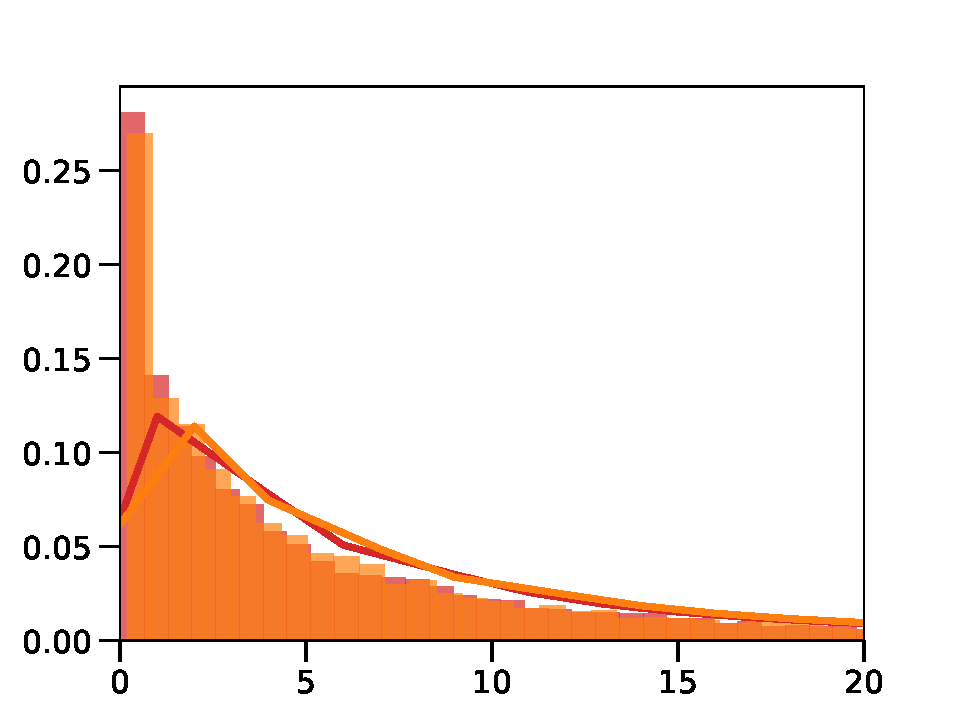
\includegraphics[scale=0.39]{figS4a_blank.pdf}};
   		\begin{scope}[x=(Bild.south east),y=(Bild.north west)]
        	\draw (0.5,-0.035) node {extinction time (days)};
        	\draw (-0.02,0.5) node [rotate=90] {probability density};

        	\draw[nred,thick] (0.325,0.8) -- node[right=6pt] {\scriptsize \color{black} increasing virus clearance $c$} (0.375,0.8);
        	\draw[orange,thick] (0.325,0.73) -- node[right=6pt] {\scriptsize \color{black} reducing infectivity $\beta$} (0.375,0.73);

        	%\draw[black,thick] (0.15,0.6) -- node[right=6pt] {\scriptsize \color{black} $V_0=1$} (0.2,0.6);
        	%\draw[black,thick,dotted] (0.15,0.53) -- node[right=6pt] {\scriptsize \color{black} $V_0 = 100$} (0.2,0.53);
			
    		\end{scope}
\end{tikzpicture}

\end{document}